\documentclass[a4paper,12pt]{report}
\usepackage[utf8]{inputenc}
\usepackage[ngerman]{babel}
\usepackage{titlesec}
\usepackage{graphicx}
\graphicspath{ {./images/} }
\usepackage{setspace}
\usepackage{lipsum}
\usepackage{geometry}
\usepackage{tocbibind}
\usepackage{dirtree}
\usepackage{hyperref}
\usepackage{array}
\usepackage{footnote}
\usepackage{natbib}
\usepackage{listings}
\usepackage{tikz}
\usetikzlibrary{positioning}
\usepackage{xcolor}
\bibliographystyle{unsrtnat}
\newcommand{\footcite}[1]{\footnotemark\footnotetext{\cite{#1}}}

\renewcommand{\lstlistingname}{Code Snippet}
\definecolor{darkgreen}{rgb}{0.0, 0.5, 0.0}
\lstdefinestyle{codeStyle}{
  language=Java, 
  basicstyle=\ttfamily\small,
  numbers=left,
  numberstyle=\tiny\color{gray},
  stepnumber=1,
  numbersep=5pt,
  showspaces=false,
  showstringspaces=false,
  showtabs=false,
  tabsize=2,
  breaklines=true,
  breakatwhitespace=true,
  stringstyle=\color{red},
  keywordstyle=\color{blue},
  commentstyle=\color{darkgreen},
  frame=single,
  rulecolor=\color{gray},
  captionpos=b,
  escapeinside={\%*}{*)},
}





\geometry{a4paper, left=25mm, right=25mm, top=30mm, bottom=30mm}

\titleformat{\chapter}{\normalfont\huge}{\thechapter.}{20pt}{\huge\bfseries}
\titleformat{\section}{\normalfont\Large}{\thesection}{12pt}{\Large\bfseries}
\titleformat{\subsection}{\normalfont\large}{\thesubsection}{8pt}{\large\bfseries}

\title{Webbasierte Multiplayer Schach-App}
\author{Jasper Paul Fülle}
\date{24. Mai 2023}

\begin{document}

\begin{titlepage}
    \begin{center}
        \vspace*{1cm}
        
        \Large
        \textbf{Webbasierte Multiplayer Schach-App}
        
        \vspace{0.5cm}
        
        Bachelorarbeit
        
        \vspace{1.5cm}
        
        \normalsize
        vorgelegt von\\
        Jasper Paul Fülle\\
        Matrikelnummer 3367654
        
        \vspace{1cm}
        
        Betreut von\\
        Prof. Dr. Thorsten Thormälen
        
        \vspace{1cm}
        
        Studiengang  Wirtschaftsinformatik 
        
        \vspace{1cm}
        
        \today
        
        \vfill
        
        
        \vspace{0.5cm}
        
        Fachbereich Mathematik und Informatik\\
        Philipps-Universität Marburg
    \end{center}
\end{titlepage}

\tableofcontents

\chapter{Einleitung}
    \section{Motivation}
    Schach ist ein traditionsreiches und abwechslungsreiches Brettspiel, deren Ursprung nicht genau bestimmt werden kann. Es wird vermutet, dass das erste schachähnliche Spiel  \textit{Tschaturanga} seinen Ursprung in Nordindien um 600 n. Chr. hatte\footcite{schachgeschichte}.
    Im Laufe der Jahrhunderte hat Schach eine bedeutende Rolle in der Kultur und Geschichte gespielt. So wurde beispielsweise die Schach-WM 1972 eine Art Machtkampf im kalten Krieg zwischen der UdSSR, welche den damaligen Schach dominierten, und der USA\footcite{bobby}.
    Schach bleibt bis heute ein beliebtes Spiel, welches 2020 durch die Netflix Serie \textit{Damengambit} und 2022 durch den Betrugsvorwurf von Magnus Carlsen an seinen 19-jährigen Gegner Hans Niemann\footcite{schachskandal} eine breitere Aufmerksamkeit erhielt (siehe Abbildung \ref{fig:Schachinteresse}). 
     Darüber hinaus hat Schach im digitalen Zeitalter eine neue Popularität erreicht. Online-Schachplattformen wie \url{chess.com} verzeichnen Milliarden von Live-Partien\footcite{chesscom3}, während Schach Live-Streams auf Plattformen wie \url{twitch.com} Millionen von Followern anziehen.
     
Die Entwicklung einer webbasierten Multiplayer-Schach-App bietet eine einzigartige Gelegenheit, ein traditionsreiches und beliebtes Spiel im digitale Zeitalter weiter zu entwickeln. Meine Motivation für diese Arbeit besteht darin, eine App zu entwickeln, die die Grundlagen einer Schach-App enthält und gleichzeitig eine solide Basis für zukünftige Erweiterungen und Verbesserungen bietet. Insbesondere plane ich, innovative Funktionen zu integrieren, die bislang in den gängigen Schach-Apps nicht vorhanden sind, wie z.B. die Möglichkeit, unterschiedliche Schachfiguren und -bretter als Belohnungen freizuschalten oder mit Freunden eine Gruppe zu gründen, welche in einer Liga auf- und absteigen kann. Durch die Entwicklung einer Schach-App mit neuen Funktionalitäten kann ich dazu beitragen, die Popularität von Schach zu steigern und vor allem das Spiel einem breiteren Publikum zugänglich zu machen.
    \section{Zielsetzung}
    Diese Bachelorarbeit hat das Ziel eine Schach-App zu entwerfen und zu implementieren, die eine intuitive User Experience und ein ansprechendes User Interface mit vielen nützlichen Funktionen beinhaltet.
    
    User Experience (\textit{UX}) bezieht sich darauf wie ein Nutzer sich auf einer Anwendung bewegt und wie einfach und angenehm es für den Nutzer ist, die Funktionen der Anwendung zu verwenden.
    
    Das User Interface (\textit{UI}) beschäftigt sich mit der visuellen und interaktiven Gestaltung von Benutzeroberflächen. Es umfasst die Gestaltung von Buttons, Formularen und anderen visuellen Komponenten, sowie das Feedback dieser Komponenten, wie zum Beispiel die Rückmeldung eines fehlgeschlagenen Logins.
    Zusammengefasst beschäftigt sich UX damit, wie man eine Anwendung verwendet und UI damit, wie die Benutzeroberfläche der Anwendung aussieht.\footcite{webdesign}
        
        Funktionen der Schach-App sind unter anderem das Registrieren und Einloggen, das Versenden, Annehmen und Ablehnen von Freundschaftsanfragen, das Zuschauen bei laufenden Spielen, das Herausfordern von Freunden zu Schachspielen und natürlich das Spielen von Schachpartien mit einem Chat und verschiedenen Einstellungsmöglichkeiten der Schach Uhren selbst.
    Dabei wird besonderer Wert auf die Verwendung moderner Web-Technologien wie React, Node.js, Socket.IO, Redis und PostgeSQL gelegt, um eine optimale Benutzererfahrung und Skalierbarkeit zu gewährleisten. Darüber hinaus soll die Arbeit einen Überblick über die technischen Herausforderungen und Lösungen im Zusammenhang mit der Implementierung einer solchen Schach-App bieten.
    
    \section{Aufbau der Arbeit}
Diese Bachelorarbeit gliedert sich in sechs Hauptkapitel, die jeweils unterschiedliche Aspekte der Entwicklung und Implementierung der Schach-App behandeln.

Im ersten Kapitel, der \textit{Einleitung}, werden die Motivation für die Entwicklung der Schach-App, die Zielsetzung der Arbeit und der Aufbau der Arbeit selbst vorgestellt.

Das zweite Kapitel, \textit{Theoretische Grundlagen}, erläutert die Grundlagen von Schach als Spiel sowie die verwendeten Web-Technologien wie Node.js, Express, Socket.io, React und PostgreSQL, die für das Verständnis der nachfolgenden Kapitel wichtig sind.

Im dritten Kapitel, \textit{Systemarchitektur}, wird die Gesamtarchitektur der Schach-App beschrieben, einschließlich der Unterteilung in Frontend und Backend, der Datenbankstruktur und der Kommunikation zwischen den verschiedenen Komponenten.

Das vierte Kapitel, \textit{Implementierung}, geht auf die praktische Umsetzung der Schach-App ein, indem es die Entwicklungsprozesse für das Frontend und das Backend sowie die Integration der Datenbanken erläutert.

Das fünfte Kapitel, \textit{Tests und Evaluation}, behandelt die verschiedenen Tests, die durchgeführt wurden, um die Funktionalität, Usability, Performance und Sicherheit der Schach-App zu bewerten.

Im abschließenden sechsten Kapitel, \textit{Fazit und Ausblick}, werden die Ergebnisse der Arbeit zusammengefasst, eventuelle Limitationen diskutiert und mögliche Erweiterungen und Weiterentwicklungen für die Schach-App vorgeschlagen.

Die Arbeit endet mit dem \textit{Anhang}, der zusätzliche Grafiken und die Liste der verwendeten Literatur enthält.
\chapter{Theoretische Grundlagen}
    \section{Schach}
   Schach ist ein strategisches Brettspiel für zwei Spieler, welches auf einem quadratischen Spielfeld mit 64 Feldern gespielt wird. Jeder Spieler beginnt mit 16 Figuren und das Ziel des Spiels ist es, den König des Gegners schachmatt zu setzen, indem man ihn bedroht, ohne dass der Gegner den Angriff verhindern kann. 
   
   Wie sich welche Figuren bewegen und andere Figuren schlagen erkläre ich nicht explizit, lediglich zwei Sonderregeln des Schachs werde ich genauer erklären, da diese bei der Umsetzung des Spiels gesondert gehandhabt werden müssen.
   
   Die erste ist das so genannte \textit{en passant}-Regel. Dabei ist es einem Bauern möglich einen gegnerischen Bauer diagonal zu schlagen, falls dieser zwei Felder gezogen ist und nun auf der gleichen Höhe wie der eigene Bauer steht (siehe Abbildung \ref{fig:en-passant}).
   
   Die zweite Zusatzregel ist die \textit{Bauernumwandlung}. Sie besagt, dass falls ein Bauer die gegnerische Grundreihe erreicht, dieser Bauer in eine Dame, einen Springer, einen Turm oder einen Läufer umgewandelt werden kann (siehe Abbildung \ref{fig:promotion}).
   
   //Schachuhr Konfigurationen erklären.
    \section{Web-Technologien}
        \subsection{Node.js und Express}
        \subsubsection{Node.js und seine Vorteile}
        \label{sec:node.js}
Node.js ist eine JavaScript-Laufzeitumgebung, welche erstmals 2009 angekündigt wurde\footcite{nodeyoutube} und speziell für die Entwicklung von skalierbaren Netzwerkanwendungen entworfen wurde\footcite{nodejs}. Skalierbarkeit bedeutet, dass mit steigender Benutzeranzahl der Ressourcenverbrauch idealerweise linear steigt. Zu den relevanten Ressourcen von Webanwendungen gehören Rechenleistung, Ein-/Ausgabeoperationen (\textit{I/O}) und Arbeitsspeicher, wobei Node.js vor allem die Skalierbarkeit von I/O intensiven Anwendungen verbessert\footcite{nodejsbook}.
I/O-Zugriffe sind beispielsweise Zugriffe auf Datenbanken, Webservices oder auf das Dateisystem. Node.js setzt dabei vollständig auf asynchrone Zugriffe. Dabei wartet der Thread nicht auf das Ergebnis eines I/O-Zugriffs, sondern führt andere Aufgaben aus, bis das Ergebnis verfügbar ist. Anschließend wird eine zuvor definierte Callback Funktion (siehe Code Snippet \ref{lst:callback}) durchgeführt. Bei einem synchronen Zugriff, wie es bei einigen anderen Laufzeitumgebungen der Fall ist, würde der Thread auf das Ergebnis warten und dieses anschließend weiterverarbeiten, wobei jedoch sein Speicherplatz zum Teil belegt bleibt. Die Vorteile hinsichtlich der Skalierbarkeit werden jedoch erst bei einer hohen Anzahl von Zugriffen erkennbar.

\begin{lstlisting}[style=codeStyle, caption={Beispiel einer Callback Funktion \textbf{Quelle: } \cite{nodejsbook}}, label={lst:callback}]
database.query(  "SELECT * FROM user",  function(result) {
result...
});
\end{lstlisting}


Ein für mich großer und entscheidender Vorteil der Nutzung von Node.js ist, ist die Nutzung der gleichen Programmiersprache für Frontend und Backend, zumal die Syntax von JavaScript mir auch schon ein wenig geläufig war.
In einem Team-Projekt kann das natürlich besonders nützlich sein, da Kommunikationsbarrieren durch unterschiedliche Programmiersprachen von Frontend und Backend niedriger sind. Natürlich versteht deshalb der Frontend-Entwickler nicht alles was  der Backend-Entwickler macht und umgekehrt, jedoch gibt es eine gemeinsame Grundlage. Neben den Kommunikationsvorteilen ermöglicht die Verwendung von der gleichen Programmiersprache im Frontend und Backend das Teilen von Code. So ist es zum Beispiel möglich Callback Funktionen vom Frontend an das Backend zu senden und dort aufzurufen.

Node.js basiert auf der Verarbeitung von Requests vom Frontend und dem zurück senden von einem Result mittels dem HTTP-Protokoll. Das HTTP-Protokoll verwendet verschiedene Methoden wie GET, POST, PUT und DELETE, um unterschiedliche Aktionen durchzuführen. Zum Beispiel wird GET zum Abrufen von Informationen verwendet, während POST zum Senden von Daten verwendet wird. Die Art und Weise wie ein Request verarbeitet werden soll ist dabei selbst zu definieren (siehe Abbildung \ref{fig:node-request}). Dabei kann der Request sein, eine bestimmte Seite zu laden, womit dann mit der entsprechenden HTML-Datei geantwortet wird, oder es kann als API genutzt werden, um Beispielsweise Daten einer Datenbank zu übermitteln. Um die Verarbeitung dieser Anfragen weniger komplex zu gestalten gibt es die Erweiterung \textit{Express} für Node.js.

\subsubsection{Express}
\label{sec:express}
\textit{Express} ist ein leichtgewichtiges und sehr beliebtes Web-Frameworks, welches unter Node.js zur Verfügung steht. Es dient zur Vereinfachung der API von Node.js und stellt hilfreiche Funktionen bereit\footcite{expressbook}. Es ermöglicht beispielsweise die Verwendung von \textit{Middleware} und \textit{Routing}.

\textit{Middleware} ermöglicht, dass eine Anfrage an den Node.js Server nicht ausschließlich von einer Funktion bearbeitet werden muss, welche das Ergebnis zurücksendet, sondern von mehreren Funktionen, die sich um verschiedene Teile der Request kümmern (siehe Abbildung \ref{fig:express-request}). Diese Funktionen heißen \textit{Middleware}. Dabei gibt es eine von uns definierte Reihenfolge der Middlewares. Zum Beispiel können wir definieren, dass zu erst der Request von einer Middleware geloggt werden soll, anschließend soll der Benutzer Authentifiziert werden. Will der Benutzer eine URL aufrufen, für die er keine Berechtigung hat wird eine \glqq not authorized\grqq{ }Seite zurück gesendet und die nächste Middleware wird nicht aufgerufen. Ansonsten wird die nächste Middleware der Kette ausgeführt, wie zum Beispiel das senden von Informationen (siehe Abbildung \ref{fig:middleware-beispiel}). Ein Vorteil der Nutzung von Middlewares ist, dass es bereits viele vordefinierte Middlewares (auch von Dritten) gibt, welche nützliche Funktionalitäten mitbringen. Die Anfrage des Frontends in mehrere kleinere Funktionen aufzuteilen, anstatt eine Funktion zu schreiben, welche sich um all dies kümmert verringert die Komplexität enorm.

\textit{Routing} hilft dabei zu identifizieren bei welchem Request welche Middleware ausgeführt	werden soll (siehe Abbildung \ref{fig:routing-beispiel}). Beispielsweise kann eine Anfrage an die URL \url{/auth} mit den angegeben Login Daten des Benutzers gesendet werden. Unter diesem Pfad können wir dann bestimmte Middlewares verwenden, welche sich mit der Authentifizierung des Benutzers befassen.
        \subsection{Socket.io}
        \label{sec:socket.io}
Die Kommunikation mit dem HTTP-Protokoll über Express hat den Nachteil, dass für jeden Datenaustausch eine neue Verbindung aufgebaut und wieder geschlossen wird, was zu einer Latenz führt, welche für Echtzeit-Anwendungen ungeeignet ist. Diese Problematik behebt das Framework \textit{socket.io}. %QUELLE BENÖTIGT%

Es ermöglicht eine direkte, bidirektionale Echtzeitübertragung von Daten mittels Websockets, long-polling und fünf anderen Protokollen zwischen den Clients und dem Server. Diese Echtzeitkommunikation ist für viele Spiele, wie auch für diese Schach-App, essentiell. So können beim Spielen mit Schachuhr Millisekunden entscheidend sein.
Neben der Echtzeitkommunikation überprüft socket.io unter anderem Timeouts, Verbindungsabbrüche, stellt Verbindungen automatisch wieder her und sorgt dafür, dass die Events in der richtigen Reihenfolge beim Server und beim Client ankommen. 

Die Kommunikation mit Socket.io läuft ausschließlich über Events. So kann man sowohl bei dem Client, als auch bei dem Server Eventlistener definieren, die auf ein bestimmtes Event hören und darauf hin eine Funktion auf den übertragenen Daten anwenden. Diese Eventlistener (definiert mit der Funktion \verb|.on()|) haben als ersten Parameter den Namen des Events als String, auf den dieser Listener hören soll und als zweiten Parameter die auszuführende Callback Funktion, welche mit den Parametern aufgerufen wird, die beim senden des Events übertragen wurden.

Events können basierend auf verschiedenen Aktionen wie zum Beispiel dem Drücken eines Buttons im Frontend oder als Reaktion eines eingegangenen Events auf dem Server gesendet werden (mit der Funktion \verb|.emit()|) (siehe Abbildung \ref{fig:socket.io-beispiel}). Der erste Parameter der \verb|emit|-Funktion ist wieder der Name des Events als String und im Anschluss kann man beliebig viele Parameter übertragen mit denen die Callback-Funktion des Listeners aufgerufen wird.

Ein wichtiges Feature von socket.io sind die Räume\footcite{socket-rooms}. Sockets im Backend können ihnen Beitreten und sie Verlassen. Serverseitig kann man dadurch an alle Sockets, die in einem bestimmten Raum sind etwas senden, ohne es allen einzeln schicken zu müssen (siehe Abbildung \ref{fig:socket.io-room}). Hier kann man sich entschließen das Event an alle clients im Raum zu versenden (\verb|io.to(...).emit(...)|) oder an alle, außer den sender (\verb|socket.to(...).emit(...)|) (siehe Code Snippet \ref{lst:socket-rooms}).

Des weiteren erhält jede socket beim Verbinden eine eigene ID, die ebenfalls als Raum genutzt werden kann. Dementsprechend ist \verb|io.to(socket.id).emit('hello');| äquivalent zu \verb|socket.emit('hello');|.


\begin{lstlisting}[style=codeStyle, caption={Beispiel zum Beitreten Raums und das senden eines Events in diesen Raum}, label={lst:socket-rooms}]
//Server
io.on("connection", (socket) => {
  socket.join("Chat");
  socket.on("message", (text) => {
  	socket.to("Chat").emit("message", text);
  }
  //Empfangen der Nachricht und weiterleiten an alle im Raum, ausser Sender.
});

//Frontend
...
socket.emit("message", "hello world"); //Senden
socket.on("message", text => console.log(text)); //Empfangen
...
\end{lstlisting}
//QUELLE socket.io im nodejsbook
        \subsection{React}
        \label{sec:react}
React ist eine der beliebtesten (nach einer Umfrage von 2022 von Stack Overflow sogar die beliebteste\footcite{stack-overflow-survey}) Frontend Javascript Bibliotheken. Es basiert auf Komponenten, welche wiederverwendbar und kombinierbar sind und vereinfacht die Verwaltung von Interaktionen mit User Interfaces. Dabei benutzt React eine Syntax Erweiterung namens \textit{JSX}. Mit dieser Erweiterung ist es möglich HTML Elemente in JavaScript Dateien zu verwenden, welches es ermöglicht die Logik hinter getrennten HTML und JavaScript Dateien in eine Datei zu kombinieren. Die Idee hinter React ist, dass wenn sich nur ein bestimmter Teil des User Interfaces im Vergleich zum aktuell sichtbaren User Interface ändert, auch nur dieser Teil neu gerendert wird und nicht das ganze User Interface. Diese reaktiven Änderungen veranlasst React mittels seiner \textit{Hooks}.

Ich werde die Art und Weise wie React und seine Hooks funktionieren an dem Beispiel \ref{lst:react-example} erklären.
In diesem Beispiel implementieren wir die Komponente \textit{ExampleComponent}, welche zum Beispiel mittels dem Tag \verb|<ExampleComponent initialCount={10} loadingDelay={3000} />| verwendet werden kann. 

Die zwei übergebenen Variablen \textit{initialCount} und \textit{loadingDelay} werden auch \textbf{props} genannt, welche in der Komponente verwendet werden können. Eine Komponente ist eine Funktion, welche als Rückgabe den HTML-Code hat, welcher angezeigt werden soll.

Die Komponente hat den lokalen State \textit{count}, welchen wir mittels der \textbf{useState} Hook initialisieren. Die Funktion \textit{useState} nimmt als Argument den initialen Wert des States und gibt uns zwei Elemente zurück, einmal die sich verändernde State Variable \textit{count} und die Funktion \textit{setCount}, um einen neuen Wert in den State \textit{count} zu schreiben. Der zurückgegebenen Funktion \textit{setCount} kann entweder ein konkreter Wert übergeben werden, oder aber eine Funktion welche beschreibt wie der neue Wert sich aus dem alten Wert bilden soll (siehe Zeile 31 in Beispiel \ref{lst:react-example}).

Die Hook \textbf{useEffekt} nimmt zwei Argumente, eine Funktion und ein sogenanntes \textit{Dependency Array}. Das Array enthält Variablen, deren Wertänderung das Ausführen der übergebenen Funktion auslöst. So wird in unserem Beispiel die Funktion einmal beim ersten Rendern der Komponente und dann bei jeder Änderung von \textit{count} oder dem prop \textit{loadingDelay} ausgeführt. Dadurch bleibt der Titel dieser Beispiel Webanwendung immer konsistent mit dem aktuellen \textit{count} State. Als Rückgabe kann die übergebene Funktion eine weitere Funktion haben, welche ausgeführt wird, sobald die Komponente \textit{unmounted} wird. Das ist eine Phase im Lebenszyklus einer Komponente, die ausgeführt wird, sobald eine Komponente nicht mehr angezeigt wird, weil zum Beispiel auf eine andere Unterseite navigiert wird. In unserem Fall soll dann der Titel der Webanwendung nicht mehr den aktuellen Count repräsentieren, sondern \glqq React App\grqq .

\textbf{useCallback} ist eine Hook, welche unnötige Code Ausführungen vermeidet und daher ausschließlich performante Vorteile bietet. Sie nimmt die gleichen Argumente wie die \textit{useEffect} Hook und durch sie können wir eine Funktion definieren, welche nur neu initialisiert wird, falls sich eine der Variablen im \textit{Dependency Array} ändert. Würden wir sie als reguläre JavaScript Funktion definieren, würde immer wenn die Komponente gerendert wird die Funktion neu initialisiert werden.

Ein weiteres wichtiges Konzept in React ist der \textit{Context}. Mit ihm lassen sich Daten über mehrere Ebenen von verschachtelten Komponenten verfügbar machen, ohne dass man sie explizit als Prop an alle Komponenten weitergeben muss. Ein Kontext lässt sich mittels der Hook \textbf{useContext} importieren. In unserem Beispiel verwenden wir ihn um ein ThemeContext zu importieren und je nach theme ändern wir die Hintergrundfarbe unserer Komponente (siehe Zeile 35 in Beispiel \ref{lst:react-example}).

In der Rückgabe der Komponente können wir nicht nur HTML, sondern auch JavaScript innerhalb von geschweiften Klammern verwenden. So prüfen wir in unserem Beispiel mit dem ternären Operator den Wert von \textit{isLoading} und zeigen entsprechende Elemente an (siehe Zeilen 36-44, Beispiel \ref{lst:react-example}).

//ROUTER noch erklären
%react-key-concepts
\begin{lstlisting}[style=codeStyle, caption={Beispiel einer React Komponente}, label={lst:react-example}]
import React, { useState, useEffect, useCallback, useContext } from "react";

// Beispiel Context
const ThemeContext = React.createContext({ theme: "light" });

// Beispiel Component Props
function ExampleComponent({ initialCount, loadingDelay }) {
  // Beispiel useState
  const [count, setCount] = useState(initialCount || 0);
  const [isLoading, setIsLoading] = useState(true);

  // Beispiel useContext
  const { theme } = useContext(ThemeContext);

  // Beispiel useEffect
  useEffect(() => {
    document.title = `Count: ${count}`;

    const timer = setTimeout(() => {
      setIsLoading(false);
    }, loadingDelay || 2000);

    return () => {
      document.title = "React App";
      clearTimeout(timer);
    };
  }, [count, loadingDelay]);
  
  // Beispiel useCallback
  const incrementCount = useCallback(() => {
    setCount((prevCount) => prevCount + 1);
  }, []);

  return (
    <div style={{ backgroundColor: theme === "light" ? "#fff" : "#333" }}>
      {isLoading ? (
        <p>Loading...</p>
      ) : (
        <>
          <p>Count: {count}</p>
          <button onClick={incrementCount}>Increment count</button>
        </>
      )}
    </div>
  );
}

export default ExampleComponent;
\end{lstlisting}
        \subsection{PostgreSQL und Redis}
        \subsubsection{PostgreSQL}
        \label{sec:PostgreSQL}
PostgreSQL ist ein Objektrelationales Open-Source Datenbanksystem, welches erstmals 1989 veröffentlicht wurde\footcite{postgresql-book}. Die Verwaltung von Datenbanken basiert auf sogenannte Datenbankmanagementsystemen (DBMS). Das beliebteste DBMS für PostgreSQL ist \textit{pgAdmin}\footcite{pgAdmin}.  In relationalen Datenbanken sind Daten in Tabellen organisiert. Zur Bearbeitung und Auswertung von solchen Datenbanken wird die Structured Query Language (\textbf{SQL}) verwendet, die in drei Bereiche unterteilt ist\footcite{sql-book}:
\begin{itemize}
 \item Data Definition Language (DDL): Um Datenbanken, Tabellen und ihren Strukturen anzulegen, zu ändern und zu löschen.
 \item  Data Manipulation Language (DML): Zum Einfügen, Ändern, Löschen und Aktualisieren von Daten in Tabellen.
 \item Data Control Language (DCL): Zur Administration von Datenbanken
\end{itemize}

Tabellen bestehen aus Zeilen, die als Tupel bezeichnet werden, und Spalten, die als Attribute bezeichnet werden. Jedes Attribut hat einen bestimmten, von uns definierten Wertebereich, beispielsweise kann ein Attribut \glqq Preis\grqq{ }eine Zahl mit zwei Nachkommastellen oder ein Attribut \glqq Name\grqq{ }eine Zeichenkette mit maximal 20 Zeichen sein.  Attributen können bestimme Restriktionen (auch \textit{Constraints} genannt) zugewiesen werden, wie zum Beispiel die UNIQUE Restriktion, welche definiert, dass jeder Wert des Attributs nur einmal vorkommen darf.
Ein weiteres wichtiges Konzept sind Primär- und Fremdschlüssel. Mit Hilfe von ihnen können Tupel verschiedener Tabellen in Beziehung gebracht werden. Ein Primärschlüssel ist ein Attribut, welches jeden Tupel einer Tabelle eindeutig identifiziert und welches als Fremdschlüssel in anderen Tabellen referenziert werden kann. Als Beispiel könnte eine Artikelnummer in einer Tabelle der Artikel als Primärschlüssel genutzt werden, welche in einer Tabelle Rechnung mit verschiedenen abgeschlossenen Bestellungen als Fremdschlüssel referenziert werden kann.

Zudem ist PostgreSQL ACID-konform. \textbf{ACID} steht für folgende Fachbegriffe\footcite{sql-book}:
\begin{itemize}
 \item \textit{Atomicity (Atomarität)}: eine Transaktion, wie das Einfügen eines Tupels oder das Erstellen einer Tabelle, wird entweder ganz oder gar nicht ausgeführt.
 \item \textit{Consistency (Konsistenz)}: Sicherstellung, dass die Datenbank immer in einem konsistenten Zustand ist, auch wenn eine Transaktion unter- oder abgebrochen wird.
 \item \textit{Isolation}: Während einer Transaktion wird die Datenbank isoliert, da während einer Transaktion ein inkonsistenter Zustand herrschen kann. Diese Isolation wird am Ende der Transaktion aufgehoben.
  \item \textit{Durability (Dauerhaftigkeit)}: Nach einer abgeschlossenen Transaktion sind die Änderungen an der Datenbank dauerhaft abgespeichert, sodass beispielsweise ein Systemabsturz die Daten nicht gefährden kann.
\end{itemize}

In Node.js kann auf eine PostgreSQL Datenbank mittels dem Framework \textit{node-postgres} zugegriffen werden\footcite{node-postgres}.
        \subsubsection{Redis}
        \label{sec:redis}
Redis ist eine No-SQL (Not only SQL) Datenbank, welche nicht wie relationale Datenbanken auf Tabellen basieren, sondern in diesem Fall auf \textit{Key-Value}-Paaren. Redis zeichnet sich vor allem durch seine verschiedenen Datentypen und seine schnellen Schreib- und Lesevorgänge aus, welche durch die Speicherung in den Arbeitsspeicher resultieren\footcite{redis-book}. Daher ist es gut für Daten geeignet, welche eine hohe Speicherungs- oder Abruffrequenz haben. Obwohl Redis hauptsächlich im Arbeitsspeicher arbeitet bietet es auch Optionen zur Datensicherung auf der Festplatte, um Datenverluste zu vermeiden. Oft dient Redis als Cache-Speicher um häufig verwendete Daten temporär zu speichern und dadurch den Zugriff auf die Daten zu beschleunigen\footcite{redis}. 

Zu den möglichen Datentypen zählen Strings, Listen, Sets, Hashes, sortierte Sets, Streams und einige weitere\footcite{redis}. 	

 Zudem ermöglicht Redis eine gute Skalierbarkeit indem mehrere Redis Instanzen verbunden werden, anstatt eine Instanz hoch zu skalieren.
       
        \subsection{Weitere verwendete Bibliotheken}
        \label{sec:weiteres}
        \subsubsection{JWT}
        \label{sec:JWT}
JWT (\textit{JSON Web Token}) ist ein offener Standard, der eine sichere Möglichkeit bietet Informationen in Form eines JSON Objekts zu übertragen\footcite{JWT}. Diesen Informationen kann vertraut werden, da sie mittels eines privaten Server seitigen secrets mit verschiedenen Algorithmen  verschlüsselt (\textit{signiert}) und wieder entschlüsselt werden (siehe Abbildung \ref{fig:jwt-example}). Der meist verwendete Anwendungsbereich für JSON Web Tokens ist die Authentifizierung, bei der der vom Backend generierte Token in einer Session oder einem Cookie gespeichert wird. Dieser kann beim Laden einer Seite aus dem HTTP Request entnommen und mittels des secrets verifiziert werden. Dabei ist wichtig zu beachten, dass der Token nicht Client seitig manipulierbar sein darf, da das ein Sicherheitsrisiko darstellen kann. Dies kann beispielsweise mit einem HTTP-Only Cookie\footcite{Http-only} erreicht werden.
 
        \subsubsection{Chakra UI}
        \label{sec:chakraUI}
Chakra UI ist eine simple Komponenten Bibliothek, welche das designen von React Anwendungen vereinfacht\footcite{chakraui}. Es stellt Komponenten zur Verfügung, welchen verschiedene Attribute zugeordnet werden können um diese nach eigenem ermessen zu designen (siehe Code Beispiel \ref{lst:chakra-example} und Abbildung \ref{fig:chakra-example}).

\begin{lstlisting}[style=codeStyle, caption={Beispiel mit Chakra UI designten React Komponente (siehe Abbildung  \textbf{Quelle: } \cite{chakraui}}, label={lst:chakra-example}]
import * as React from "react";
import { Box, Center, Image, Flex, Badge, Text } from "@chakra-ui/react";
import { MdStar } from "react-icons/md";

export default function Example() {
  return (
    <Center h="100vh">
      <Box p="5" maxW="320px" borderWidth="1px">
        <Image borderRadius="md" src="https://bit.ly/2k1H1t6" />
        <Flex align="baseline" mt={2}>
          <Badge colorScheme="pink">Plus</Badge>
          <Text
            ml={2}
            textTransform="uppercase"
            fontSize="sm"
            fontWeight="bold"
            color="pink.800"
          >
            Verified &bull; Cape Town
          </Text>
        </Flex>
        <Text mt={2} fontSize="xl" fontWeight="semibold" lineHeight="short">
          Modern, Chic Penthouse with Mountain, City & Sea Views
        </Text>
        <Text mt={2}>$119/night</Text>
        <Flex mt={2} align="center">
          <Box as={MdStar} color="orange.400" />
          <Text ml={1} fontSize="sm">
            <b>4.84</b> (190)
          </Text>
        </Flex>
      </Box>
    </Center>
  );
}
\end{lstlisting}
        \subsubsection{Formik und Yup}
        \label{sec:formik}
Formik ist die beliebteste Open-Source-Bibliothek für Formulare in React \footcite{formik}. Sie vereinfacht die Handhabung von Formularen und bietet Funktionen wie Validierung der eingegebenen Werte, Fehlermeldungen und Unterstützung für mehrstufige Formulare.

Yup ist eine Bibliothek  zur einfachen Definition von Schemata, die von bestimmten Formularen erfüllt werden sollen. Sie ermöglicht die Erstellung komplexer Schemata mit wenig Code\footcite{Yup}.

Die Integration von Yup-Schemata in Formik-Formulare ist bereits unterstützt, was eine einfache Handhabung von Überprüfungen und Fehlerbehandlungen bei Benutzereingaben ermöglicht.

        \subsubsection{chess.js}
        \label{sec:chess.js}
Chess.js ist eine Schach Bibliothek, welche die gesamte Schachlogik zur Verfügung stellt\footcite{chessjs}. Es bietet Methoden, welche alle aktuell möglichen Züge ausgibt, einen Zug ausführt und verschiedene Notationen des Zuges zurückgibt, überprüft ob es sich um ein Schachmatt oder Patt handelt, eine Partie mittels einer FEN\footcite{FEN} oder PGN\footcite{PGN} Notation laden kann und vieles weitere. 
        \subsubsection{chessground}
        \label{sec:chessground}
Chessground ist ein Open-Source-Schach-User-Interface, das ursprünglich für die Online-Schachplattform \url{lichess.org} entwickelt wurde\footcite{chessground}. Es bietet zahlreiche Konfigurationsmöglichkeiten, wie zum Beispiel Animationen beim bewegen von Figuren, Auswahl der anklickbaren und bewegbaren Figuren, Anpassung des Figurendesigns und vieles mehr. Die eigentliche Schachlogik ist nicht enthalten, sodass verschiedene Schachvarianten mit Sonderregelungen implementiert werden können.
        
        
\chapter{Systemarchitektur}
Die Anwendung ist in zwei Hauptkomponenten unterteilt: das Frontend und das Backend. Das Frontend ist für die Darstellung der Benutzeroberfläche und die Interaktion mit dem Benutzer verantwortlich, während das Backend die Spiellogik, die Verwaltung der Benutzerdaten und die Echtzeit-Kommunikation zwischen den Spielern steuert.

Die Anwendung verwendet moderne Web-Technologien, um eine reaktive und benutzerfreundliche Oberfläche zu schaffen. Das Frontend basiert auf dem React-Framework\footcite{react}, das es ermöglicht, wiederverwendbare Komponenten zu entwickeln und den Anwendungsstatus effizient zu verwalten. Das User-Interface basiert auf Chakra UI\footcite{chakraui}, einem modernen und flexiblen Komponenten-Bibliothekssystem, das die Entwicklung von responsiven und zugänglichen Benutzeroberflächen erleichtert. Die Benutzerführung und die Kommunikation zwischen den React-Komponenten sind so gestaltet, dass sie eine nahtlose und intuitive Benutzererfahrung bieten.

Auf der Backend-Seite wird Node.js\footcite{nodejs} mit dem Express-Framework verwendet, um einen leistungsstarken und skalierbaren Server bereitzustellen. Die API-Endpunkte und die Kommunikation mittels WebSockets is so konzipiert, dass sie den Anforderungen der verschiedenen Frontend-Komponenten gerecht werden und die Kommunikation zwischen Frontend und Backend erleichtern. Die Echtzeit-Kommunikation zwischen den Spielern wird mit Hilfe von Socket.io\footcite{socketio} ermöglicht, einer Bibliothek, die bidirektionale Kommunikation über WebSockets unterstützt. Für die Speicherung und Verwaltung der Benutzerdaten zum Anmelden wird eine PostgreSQL\footcite{postgresql}-Datenbank verwendet, die aufgrund ihrer Leistungsfähigkeit und Flexibilität ausgewählt wurde. Freundeslisten und Daten aktiver Spiele werden in einer Redis\footcite{redis}-Datenbank gespeichert, die sich durch hohe Leistung und niedrige Latenz auszeichnet, insbesondere bei Lese- und Schreibvorgängen. Redis, eine In-Memory-Datenstruktur, eignet sich ideal für Anwendungen, bei denen schnelle Zugriffszeiten und Skalierbarkeit wichtig sind. Die Kombination von PostgreSQL und Redis ermöglicht eine effiziente Verwaltung sowohl persistenter als auch flüchtiger Daten und fördert eine optimale Benutzererfahrung.
    \section{Frontend}
Das Frontend der Anwendung wurde unter Verwendung von React (Abschnitt \ref{sec:react}), Socket.io (Abschnitt \ref{sec:socket.io}) und weiteren Bibliotheken aus Abschnitt \ref{sec:weiteres} entwickelt.

\begin{figure}[h]
\centering

\begin{minipage}{0.6\textwidth}
\dirtree{%
.1 client/.
.2 public/.
.3 Gambit dark.png.
.3 Gambit light.png.
.3 Gambit springer.png.
.3 index.html.
.3 manifest.json.
.3 robots.txt.
.2 src/.
.3 components/.
.4 ActiveGames.js.
.4 AddFriendModal.js.
.4 Chat.js.
.4 ChessClock.js.
.4 Friend.js.
.4 FriendList.js.
.4 FriendRequest.js.
.4 GameRequests.js.
.4 Navbar.js.
.4 PromotionModal.js.
.3 contexts/.
.4 AccountContext.js.
.4 SocketContext.js.
.4 tests/.
.3 themes/.
.4 Theme.js.
.3 utils/.
.4 ChessLogic.js.
.3 views/.
.4 ChessGame.js.
.4 Home.js.
.4 Login.js.
.4 Signup.js.
.3 App.js.
.3 index.js.
.3 Views.js.
.2 package.json.
}
\end{minipage}
\caption{Ordnerstruktur des Frontends}
\label{fig:frontend_dirtree}

\end{figure}

Die Ordnerstruktur (Abbildung \ref{fig:frontend_dirtree}) ist wie folgt aufgebaut:
\begin{itemize}
\item \textbf{public:} In diesem Ordner befinden sich statische Ressourcen, wie zum Beispiel Bilder des Logos, die von der Anwendung verwendet werden.
\item \textbf{components:} Dieser Ordner enthält alle React-Komponenten, die für die Anwendung verwendet werden. Sie sind modular und stellen jeweils nur ein Teil eines User Interfaces dar.
\item \textbf{contexts:} Hier befinden sich die React Contexts, die zum Verwalten von globalen Zuständen und Kommunikationsschnittstellen verwendet werden.
\item \textbf{themes:} Dieser Ordner enthält Dateien, die für das Design und die Anpassung des Aussehens der Anwendung mittels Chakra UI verantwortlich sind.
\item \textbf{utils:} In diesem Ordner befinden sich Hilfsdateien, die ausgelagerte Funktionen zur Verfügung stellen.
\item \textbf{views:} Dieser Ordner enthält die verschiedenen Seiten der Anwendung. Zu diese Seiten kann mit Hilfe des React-Routers über verschiedene URLs navigiert werden. Diese Seiten verwenden teilweise die Komponenten aus dem components-Ordner, um eine vollständige Benutzeroberfläche darzustellen.
\end{itemize}
    
        \subsection{React-Komponenten}
Der hierarchische Aufbau der React-Komponenten in Abbildung \ref{fig:frontend_tikz} zeigt die Struktur der Anwendung für eingeloggte User. Nicht eingeloggte Benutzer sehen lediglich die Komponenten ActiveGames und FriendList nicht, während der restliche Aufbau gleich bleibt. In diesem Abschnitt werden die wichtigsten Komponenten und ihre Funktionen innerhalb der Anwendung erläutert.
        
\begin{itemize}
\item \textbf{AccountContext:} Stellt Informationen über den Benutzerstatus allen Folgenden Komponenten mittels eines Contexts zur Verfügung. Diese Informationen beinhalten, ob ein Benutzer angemeldet ist und falls er das ist seinen Usernamen.
\item \textbf{SocketContext:} In diesem React Context wird eine socket.io Verbindung mit dem Server hergestellt und allen darauf folgenden Komponenten bereitgestellt.
\item \textbf{ChakraBaseProvider und ColorModeScript:} Diese importierten Komponenten von ChakraUI stellen die Funktionen zum designen bereit. Dazu gehören Beispielsweise das Verwenden des globalen Zustands des Farbenschemas (dunkel oder hell) oder das zugreifen auf definierte Stile in der themes.js Datei, welche wir den beiden Komponenten übergeben.
\item \textbf{Views:} Diese Komponente beinhaltet das User Interface. Mit Hilfe des React-Routers werden hier die Komponenten des \verb|view|-Ordners unter einem bestimmten Pfad definiert. Des weiteren beinhaltet es die Komponenten GameRequest und Navbar, welche durch die Definition in dieser Komponente auf jedem Pfad vorhanden sind.
\begin{itemize}
\item \textbf{Navbar:} Die Navigationsleiste besteht aus dem Logo und einem Button zum wechseln des Farbschemas. Je nachdem, ob ein Benutzer angemeldet ist oder nicht beinhaltet es noch Buttons zum Anmelden, Registrieren oder Abmelden (siehe Abbildungen \ref{fig:home-not-logged-in} \& \ref{fig:home-logged-in}).
\item \textbf{GameRequests:} Diese Komponente ist dafür Verantwortlich beim Eingang einer Spiel Anfrage eines Freundes, dieses als Modal darzustellen und bietet die Möglichkeit diese Anfrage zu beantworten (siehe Abbildung \ref{fig:game-request}).
\end{itemize}
\item \textbf{Home:} Diese Komponente stellt die Startseite dar und enthält die Buttons zum Starten eines Spiels mit verschiedenen Schachuhr Konfigurationen (siehe Abbildung \ref{fig:home-not-logged-in}). Ist ein Benutzer angemeldet sind auch noch die Komponenten ActiveGames und FriendList auf der rechten Seite vorhanden (siehe Abbildung \ref{fig:home-logged-in}).
\begin{itemize}
\item \textbf{ActiveGames:} ActiveGames ist eine Komponente die alle derzeit aktiven Spiele mit den Informationen der Usernames und wer welche Farbe spielt als Buttons darstellt (siehe Abbildung \ref{fig:home-logged-in}).
\item \textbf{FriendList:} Diese Komponente verwaltet alle Freunde und Freundschaftsanfragen eines Benutzers, während die Darstellung die Unterkomponenten Friend und FriendRequest übernehmen.
\begin{itemize}
\item \textbf{Friend:} Übernimmt die Darstellung eines Freundes. Mittels eines farbigen Punktes ist erkennbar, ob dieser Freund gerade online ist (grün) oder nicht (rot) (siehe Abbildung \ref{fig:home-logged-in}). Ist er online erscheint noch mindestens ein weiterer Button. Es beinhaltet ein Icon in Form von gekreuzten Schwertern und einem Schild. Dies hat die Funktion einen Freund zu einem Spiel herauszufordern. Falls dieser Freund gerade ein aktives Spiel hat erscheint noch ein zweiter Button mit einem Auge als Icon, welches den Benutzer zu dem aktiven Spiel des Freundes navigiert.
\item \textbf{FriendRequest:} Eine Freundschaftsanfrage wird mittels dieser Komponente dargestellt und beantwortet (siehe Abbildung \ref{fig:home-logged-in}).
\item \textbf{AddFriendModal:} Mit Hilfe dieser Komponente können Freundschaftsanfragen unter Angabe des Usernames versendet werden.
\end{itemize}
\end{itemize}
\item \textbf{Login \& SignUp:} Komponenten, die das Anmelden und Registrieren mittels Formularen mit Formik und Yup (siehe Abschnitt \ref{sec:formik}) ermöglichen und mit dem Server zur Authentifizierung kommunizieren. 
\item \textbf{ChessGame:} 
\begin{itemize}
\item \textbf{ChessClock:} 
\item \textbf{Chat:}
\end{itemize}
\end{itemize}
        

    
    
\begin{figure}[h]
        \centering
        \begin{tikzpicture}
\node {App}
    child {node {AccountContext}
    		child {node {SocketContext}
    			child {node {ChakraBaseProvider} [sibling distance = 2.5cm]
    				child {node [xshift= -2cm] {ColorModeScript}}
    					child {node {Views} [sibling distance = 2.6cm]
    						child {node {Home} edge from parent [dashed]					
    							child {node {ActiveGames} edge from parent [solid]}
    							child {node {FriendList} [sibling distance = 2.0cm] edge from parent [solid]
								child {node {Friend}}
    								child {node {...}}
    								child {node {FriendRequest}}
    								child {node {...}}
    								child {node {AddFriendModal}}    							
    							 }
    						}
    						child {node {Login} edge from parent [dashed]}  
    						child {node {SignUp} edge from parent [dashed]}  				
    						child {node {ChessGame} edge from parent [dashed]
						child {node {ChessClock} edge from parent [solid]}
						child {node {Chat} edge from parent [solid]}    						
    						}
						child {node {GameRequests}}
						child {node {Navbar}}  
    					}
    				} 
    			}
    		};
    		

    \node[anchor=north east, xshift=-7cm] (dashed) at (current bounding box.north east) {};
    \draw[dashed] (dashed.east) -- ++(0.8cm, 0);

    \node[anchor=west, right=1cm of dashed] {Route Komponenten};

    \node[below=0.3cm of dashed] (solid) {};
    \draw[solid] (solid.east) -- ++(0.8cm, 0);

    \node[anchor=west, right=1cm of solid] {enthaltene Unterkomponenten};
\end{tikzpicture}
    	
\caption{Aufbau der React-Komponenten für eingeloggte Benutzer}
\label{fig:frontend_tikz}
        
        \end{figure}
    
        \subsection{Benutzerführung}
        \subsection{Kommunikation mit dem Backend}
    \section{Backend}
        \subsection{API-Endpunkte}
        \subsection{Datenbankstruktur}
        		\subsubsection{PostgreSQL}
        		\subsubsection{Redis}
        \subsection{Echtzeit-Kommunikation}

\chapter{Implementierung}
    \section{Frontend-Entwicklung}
    \section{Backend-Entwicklung}
    \section{Datenbank-Integration}

\chapter{Fazit und Ausblick}
    \section{Zusammenfassung der Ergebnisse}
    \section{Limitationen}
    \section{Potenzielle Erweiterungen und Weiterentwicklung}

\appendix

\listoffigures
\begin{figure}[ht]
\raggedleft
  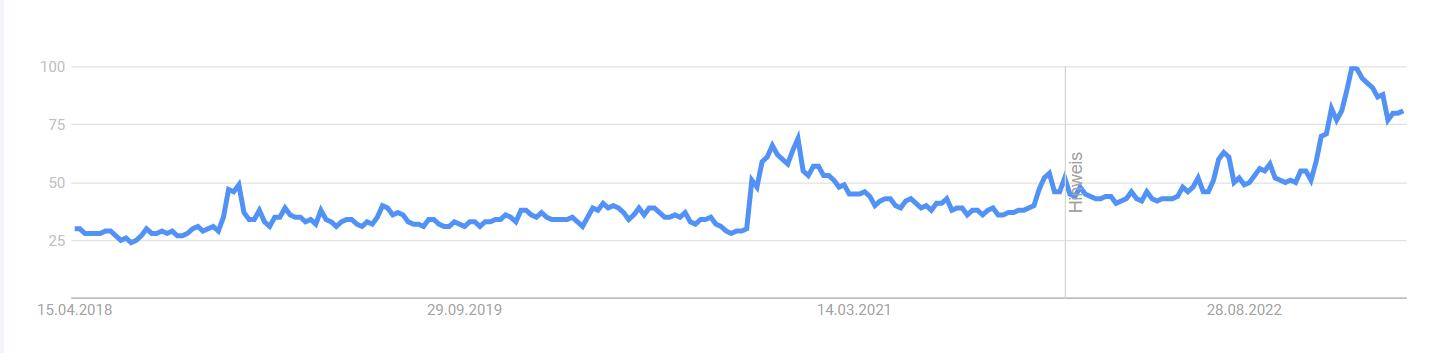
\includegraphics[width=160mm]{Schachentwicklung.jpg}
    \footnotesize\sffamily\textbf{Quelle:} \url{https://trends.google.de/}
  \caption{Relatives Suchinteresse des Wortes \textit{Chess} auf Google in den letzten 5 Jahren.}
  \label{fig:Schachinteresse}
\end{figure}
  
  \begin{figure}[ht]
\raggedleft
  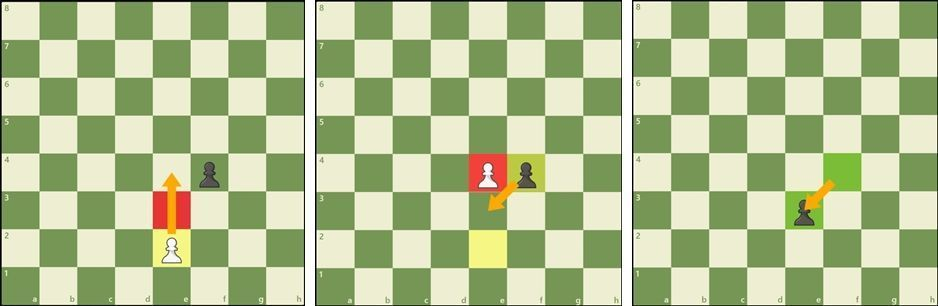
\includegraphics[width=160mm]{en-passant.jpeg}
    \footnotesize\sffamily\textbf{Quelle:} \url{https://www.chess.com/de/schachregeln}
  \caption{Die Zusatzregel \textit{en passant}}
  \label{fig:en-passant}
\end{figure}

  \begin{figure}[ht]
\centering
  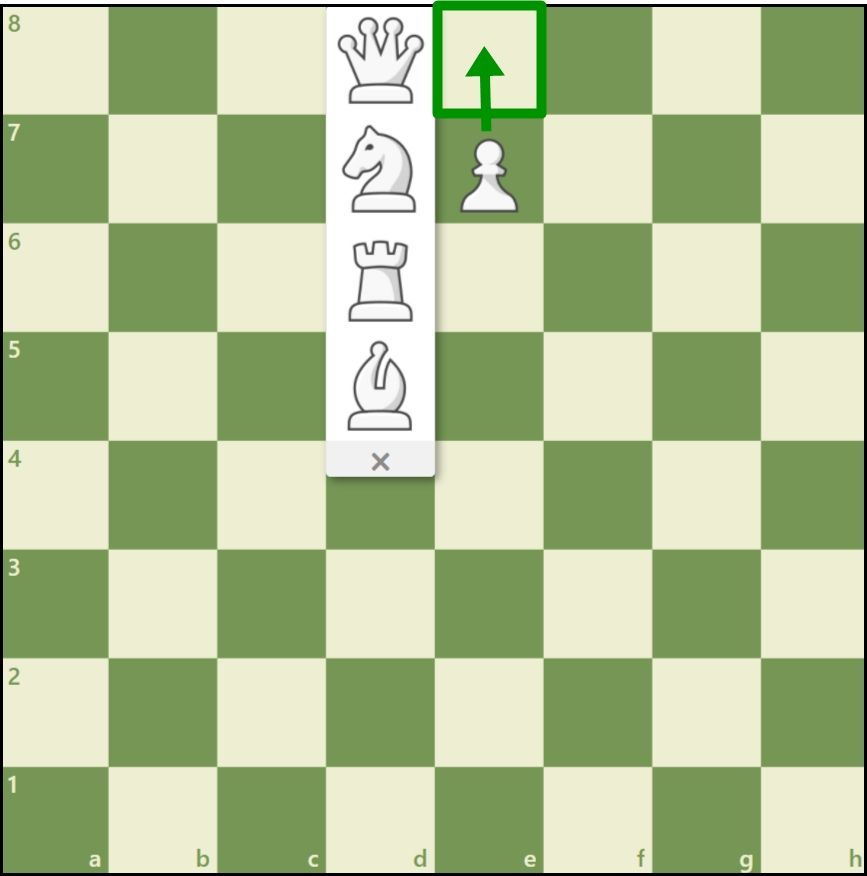
\includegraphics[height=80mm]{promotion.jpeg}
   
   
\raggedleft
    \footnotesize\sffamily\textbf{Quelle:} \url{https://www.chess.com/de/schachregeln}
  \caption{Die Zusatzregel \textit{Bauernumwandlung}}
  \label{fig:promotion}
\end{figure}

  \begin{figure}[ht]
\raggedleft
  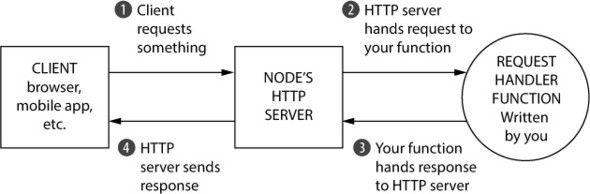
\includegraphics[width=160mm]{node-request.jpg}
    \footnotesize\sffamily\textbf{Quelle:} \cite{expressbook}
  \caption{Ablauf einer Anfrage an einen Node.js Server}
  \label{fig:node-request}
\end{figure}


  \begin{figure}[ht]
\raggedleft
  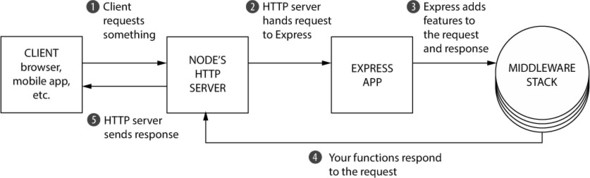
\includegraphics[width=160mm]{express-request.jpg}
    \footnotesize\sffamily\textbf{Quelle:} \cite{expressbook}
  \caption{Ablauf einer Anfrage an einen Node.js Server mit Express}
  \label{fig:express-request}
\end{figure}

  \begin{figure}[ht]
\raggedleft
  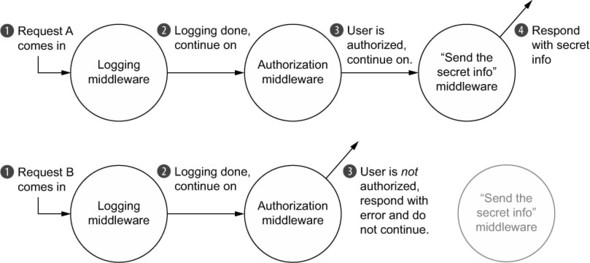
\includegraphics[width=160mm]{Middleware-Beispiel.jpg}
  
  \vspace{20mm}
  
  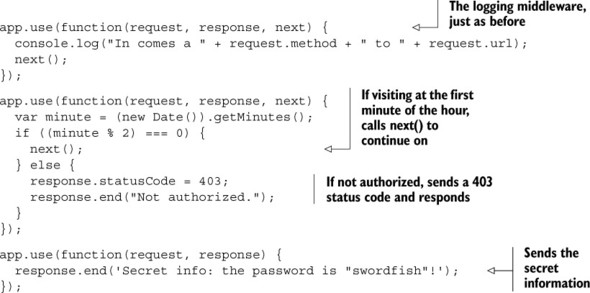
\includegraphics[width=160mm]{Middleware-Beispiel-2.jpg}
    \footnotesize\sffamily\textbf{Quelle:} \cite{expressbook}
  \caption{Beispiel der Nutzung von Middlewares}
  \label{fig:middleware-beispiel}
\end{figure}

  \begin{figure}[ht]
\raggedleft
  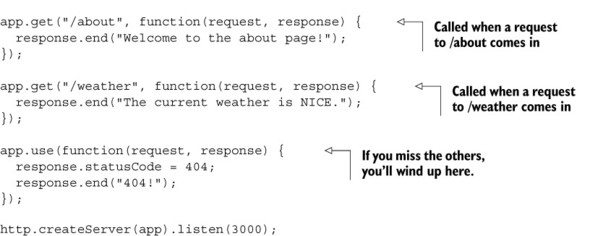
\includegraphics[width=160mm]{express-routing-example.jpg}
    \footnotesize\sffamily\textbf{Quelle:} \cite{expressbook}
  \caption{Beispiel der Nutzung von Routing}
  \label{fig:routing-beispiel}
\end{figure}

  \begin{figure}[ht]
\raggedleft
  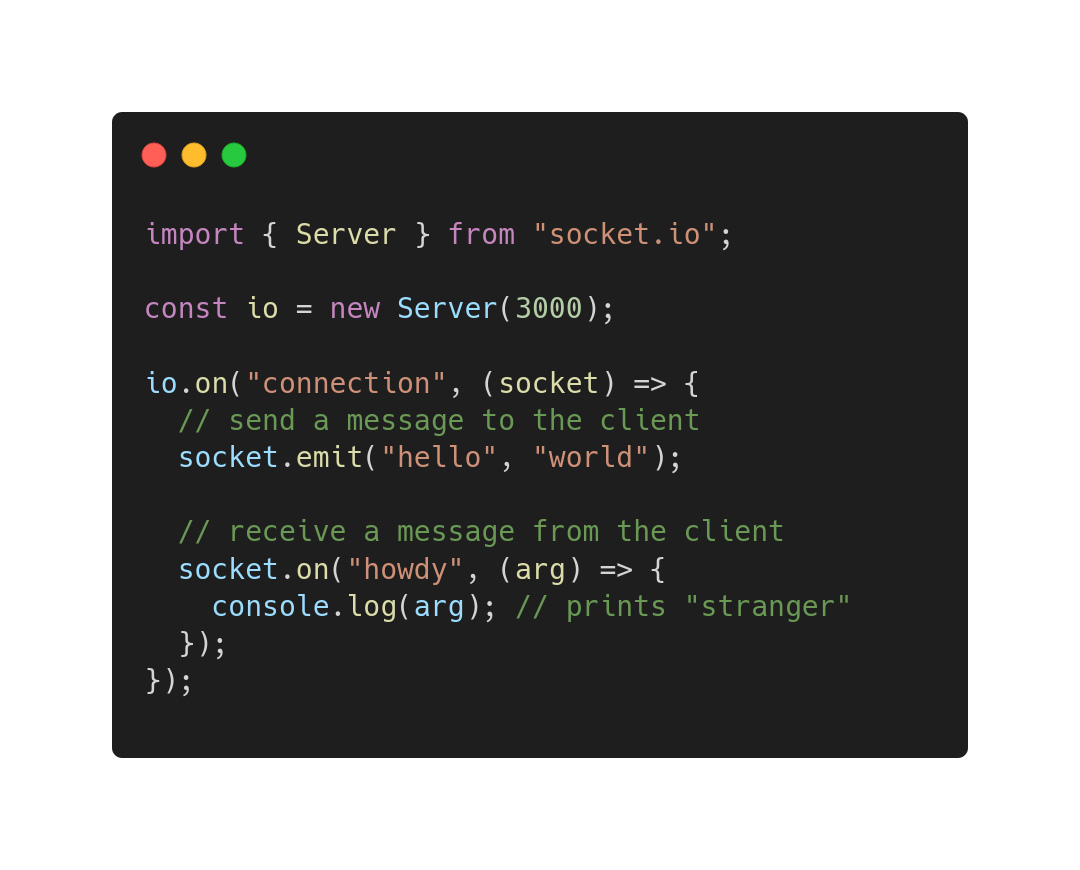
\includegraphics[width=70mm]{socket.io-server-beispiel.png}
  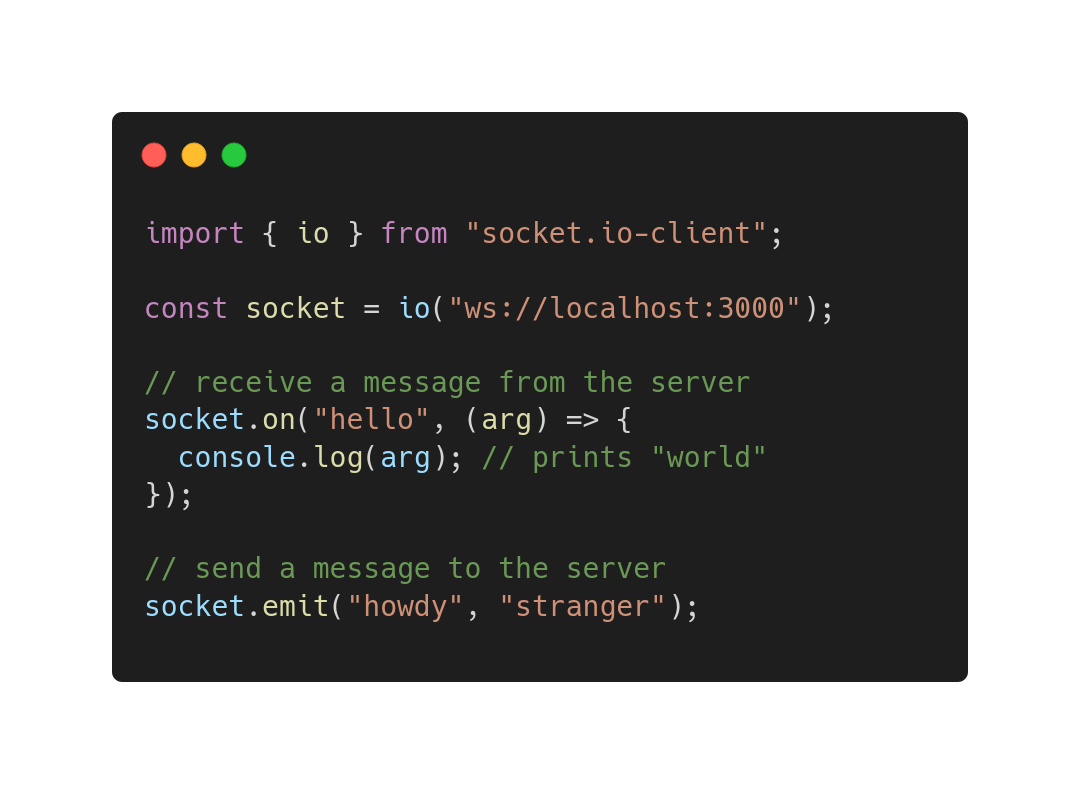
\includegraphics[width=70mm]{socket.io-client-beispiel.png}
    \footnotesize\sffamily\textbf{Quelle:} \cite{socketio}
  \caption{Simples Beispiel der Initialisierung einer socket.io Verbindung und das Senden und Empfangen von Events}
  \label{fig:socket.io-beispiel}
\end{figure}

  \begin{figure}[ht]
\raggedleft
  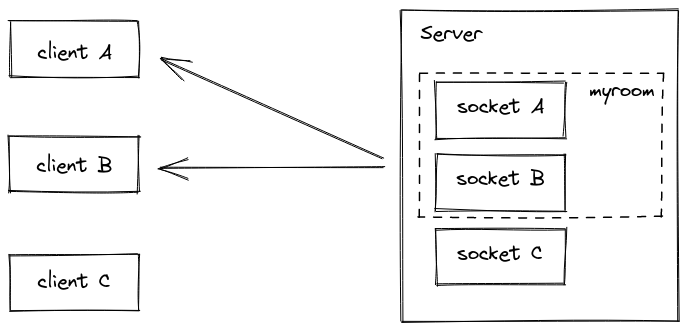
\includegraphics[width=160mm]{socket.io-rooms.png}
    \footnotesize\sffamily\textbf{Quelle:} \cite{socket-rooms}
  \caption{Darstellung eines Raumes \textit{myroom} mit zwei sockets}
  \label{fig:socket.io-room}
\end{figure}

  \begin{figure}[ht]
\raggedleft
  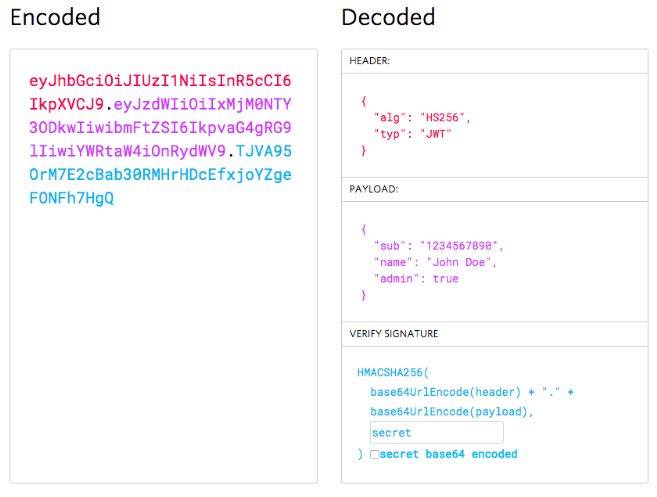
\includegraphics[width=100mm]{jwt-beispiel.png}
    \footnotesize\sffamily\textbf{Quelle:} \cite{JWT}
  \caption{Beispiel eines verschlüsselten Tokens von JWT}
  \label{fig:jwt-example}
\end{figure}

  \begin{figure}[ht]
\raggedleft
  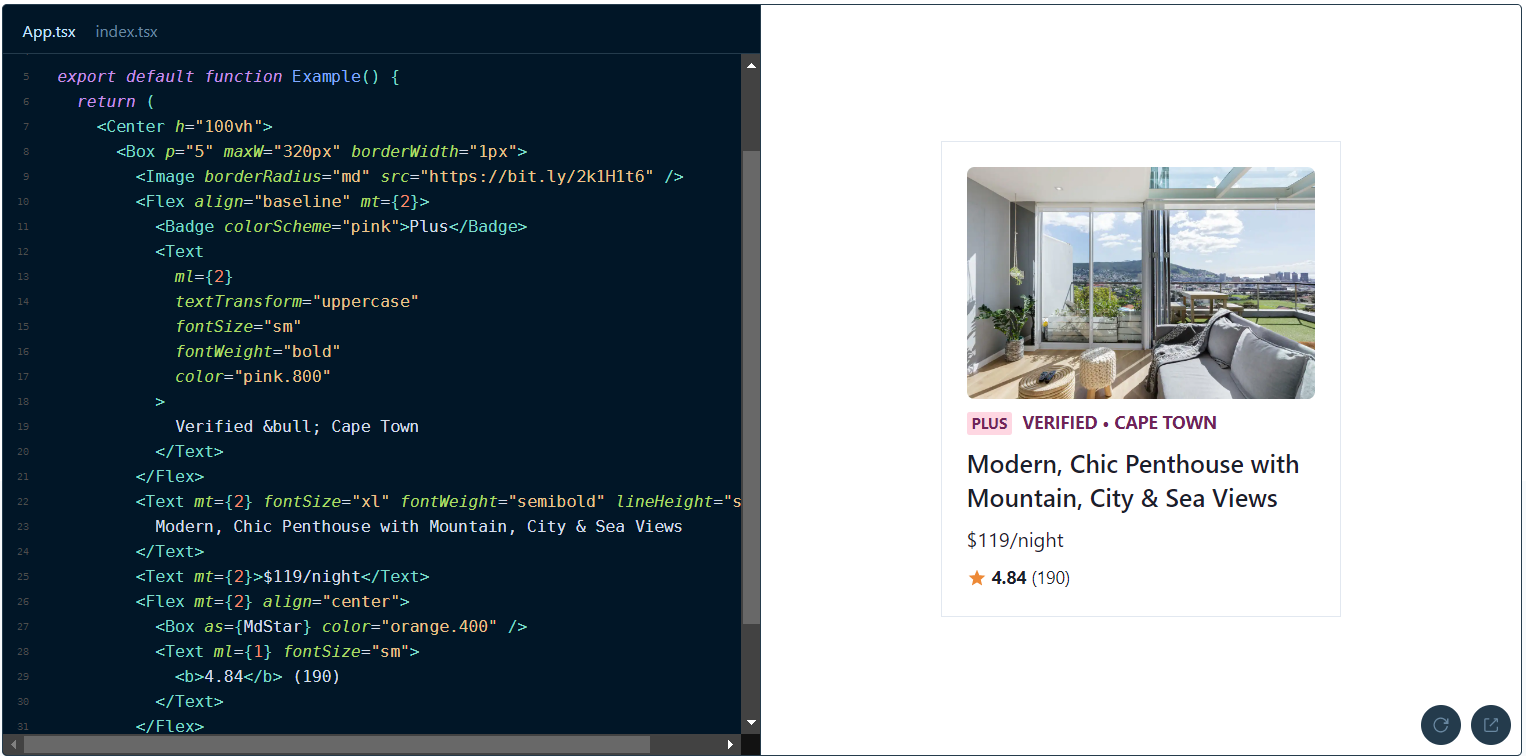
\includegraphics[width=60mm]{Chakra-UI Beispiel.png}
    \footnotesize\sffamily\textbf{Quelle:} \cite{chakraui}
  \caption{Darstellung der mit Chakra UI designten React Komponente aus dem Code Beispiel \ref{lst:chakra-example}}
  \label{fig:chakra-example}
\end{figure}
  

  \begin{figure}[ht]
\raggedleft
  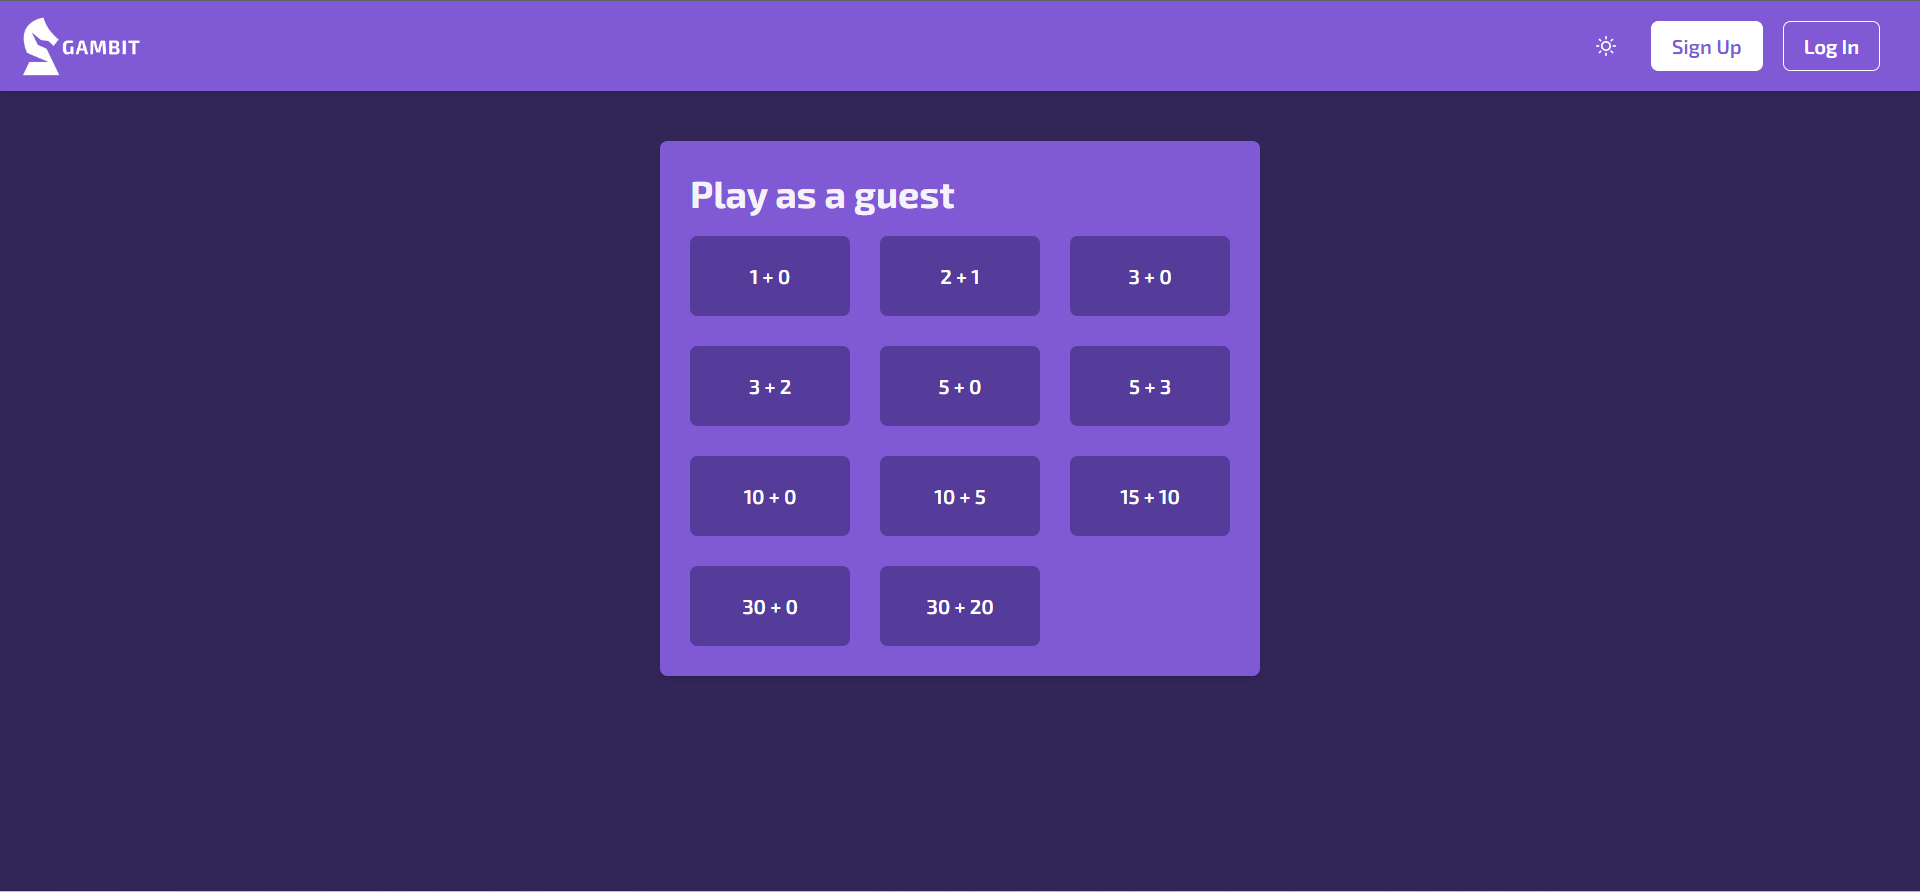
\includegraphics[width=160mm]{Home_not_logged_in.png}
  \caption{Home und Navbar Komponente eines nicht angemeldeten Benutzers im dunklen Farbschema}
  \label{fig:home-not-logged-in}
\end{figure}
  
    \begin{figure}[ht]
\raggedleft
  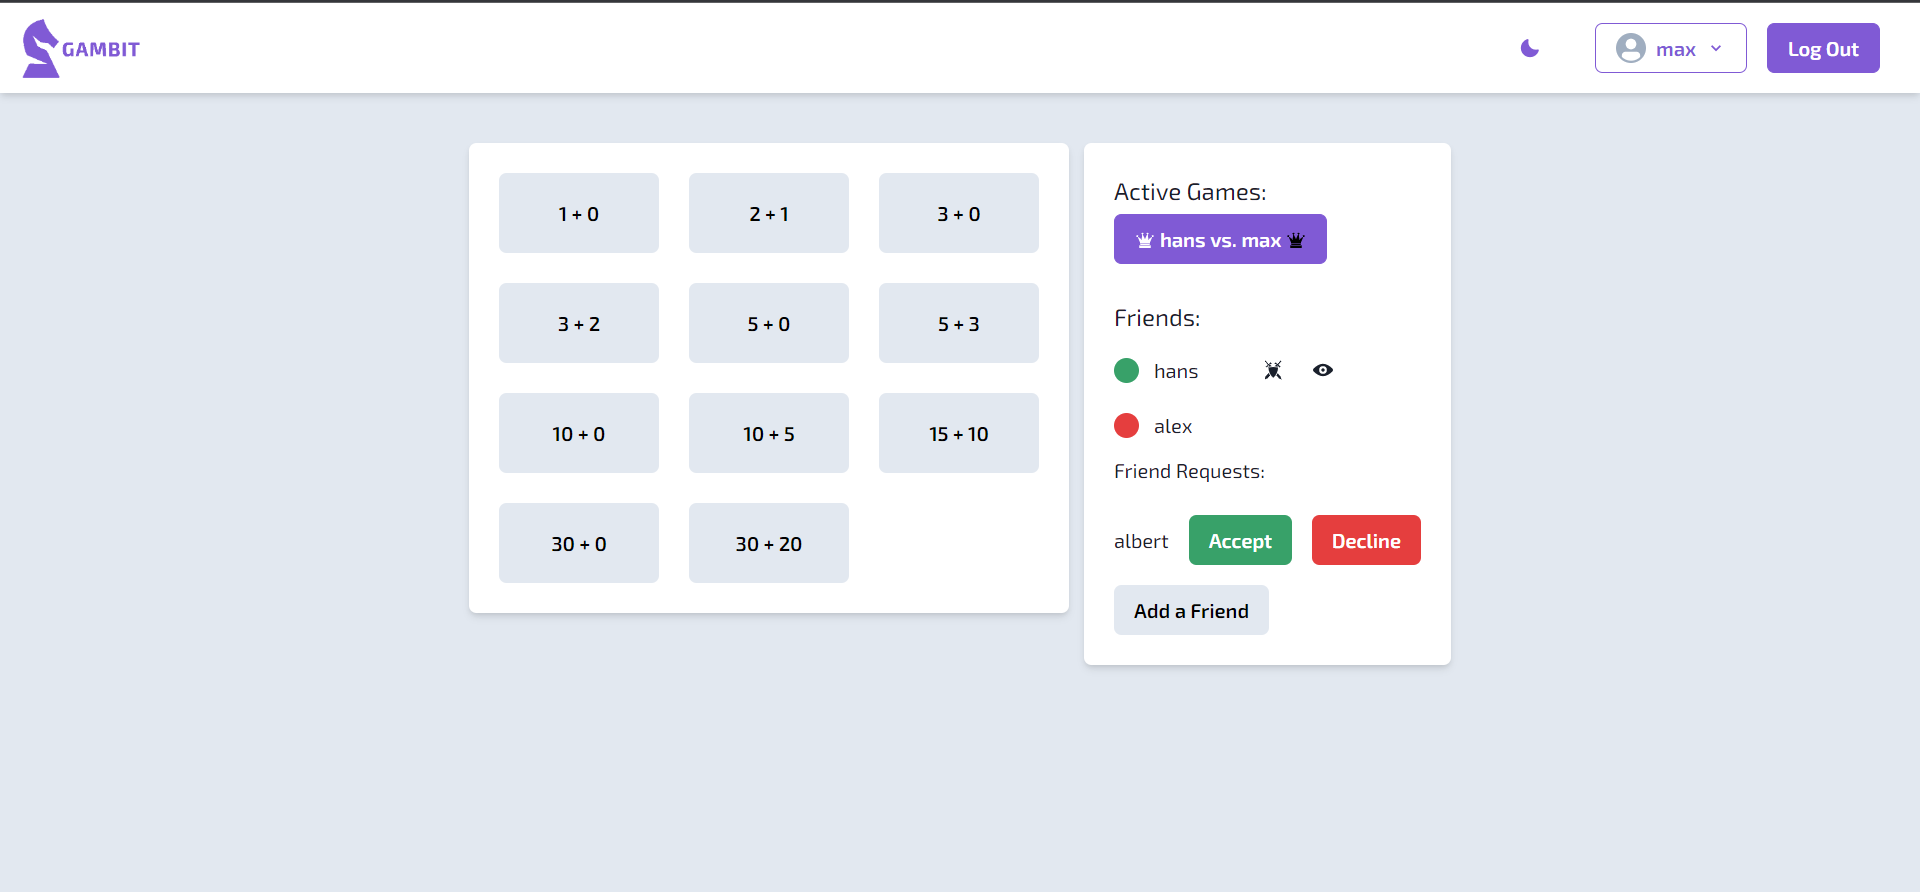
\includegraphics[width=160mm]{Home_logged_in.png}
  \caption{Home und Navbar Komponente eines angemeldeten Benutzers im hellen Farbschema}
  \label{fig:home-logged-in}
\end{figure}
  
      \begin{figure}[ht]
\raggedleft
  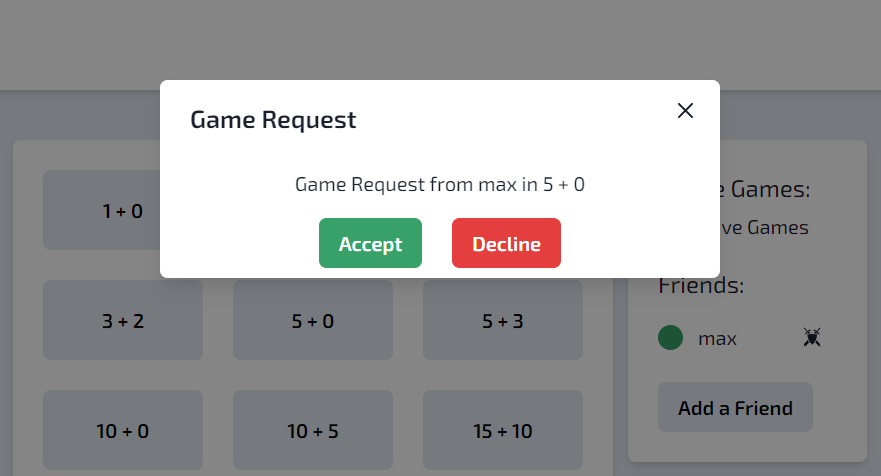
\includegraphics[width=100mm]{game_request.png}
  \caption{Das Modal der Komponente GameRequest in hellem Farbschema}
  \label{fig:game-request}
\end{figure}



\bibliography{Bibliography}

\end{document}

